\documentclass[conference]{IEEEtran}
\IEEEoverridecommandlockouts
% The preceding line is only needed to identify funding in the first footnote. If that is unneeded, please comment it out.
\usepackage{cite}
\usepackage{amsmath,amssymb,amsfonts}
\usepackage{algorithmic}
\usepackage{mathpazo}
\usepackage[spanish]{babel}
\usepackage[utf8]{inputenc}
\usepackage{graphicx}
\usepackage{textcomp}
\usepackage{xcolor}
\usepackage{adjustbox}
%\usepackage{minted}
%\usemintedstyle{emacs}
\usepackage{url}
\usepackage{ctable}
\usepackage{float}
\usepackage{amsmath,amssymb,amsfonts}
\usepackage{makecell}
\usepackage{hyperref}
\usepackage{comment}
\usepackage{tcolorbox}
\hypersetup{
	colorlinks=true,
	linkcolor=blue,
	filecolor=magenta,      
	urlcolor=cyan,
}
\newcommand{\DNoise}{n_d}

\newcommand{\Est}[1]{\hat{#1}}
\newcommand{\Test}[1]{\expandafter\hat#1}

\def\BibTeX{{\rm B\kern-.05em{\sc i\kern-.025em b}\kern-.08em
    T\kern-.1667em\lower.7ex\hbox{E}\kern-.125emX}}
    
\begin{document}
\title{\bf{Introducción a la Ciencia de Datos con Python}}
%{\footnotesize \textsuperscript{*}}

\author{
\begin{tabular}[t]{@{}c@{}}
\IEEEauthorblockN{Acurio Solar Manuel}
\IEEEauthorblockA{\textit{Escuela de Ingenieria Física} \\
\textit{Universidad Nacional de Ingeniería}\\
Lima, Perú \\
\texttt{manuel.acurio.s@uni.pe}}
\end{tabular}
\hfill
\begin{tabular}[t]{@{}c@{}}
\IEEEauthorblockN{Ahon Malca Daniel Guillermo}
\IEEEauthorblockA{\textit{Escuela de Ingenieria Física} \\
\textit{Universidad Nacional de Ingeniería}\\
Lima, Perú \\
\texttt{daniel.ahon.m@uni.pe}}
\end{tabular}
\\[1em]
\begin{tabular}[t]{@{}c@{}}
\IEEEauthorblockN{Estrada Lopez Marco Josbel}
\IEEEauthorblockA{\textit{Escuela de Física} \\
\textit{Universidad Nacional de Ingeniería}\\
Lima, Perú \\
\texttt{marco.estrada.l@uni.pe}}
\end{tabular}
\hfill
\begin{tabular}[t]{@{}c@{}}
\IEEEauthorblockN{Mozo Perez Willian Alessandro}
\IEEEauthorblockA{\textit{Escuela de Física} \\
\textit{Universidad Nacional de Ingeniería}\\
Lima, Perú \\
\texttt{willian.mozo.p@uni.pe}}
\end{tabular}
}

\maketitle

\begin{abstract}
    Este proyecto tiene como objetivo realizar un análisis exhaustivo de datos utilizando bibliotecas de Python como pandas, numpy y matplotlib. El análisis incluyó la carga y limpieza de datos, verificando y manejando valores nulos, ajustando tipos de datos y calculando estadísticas descriptivas para comprender la estructura de los datos. Posteriormente, se llevó a cabo un análisis exploratorio de datos (EDA) mediante visualizaciones como histogramas, boxplots y pairplots para explorar distribuciones y relaciones entre características, así como la creación de una matriz de correlación para identificar correlaciones entre variables. Los resultados se visualizaron mediante gráficos de dispersión y mapas de calor, proporcionando una representación clara de los hallazgos clave. Todo el proceso fue documentado adecuadamente para asegurar su reproducibilidad, con comentarios en el código y recomendaciones para el uso de herramientas como Jupyter Notebooks y sistemas de control de versiones. Este proyecto demuestra el uso de técnicas fundamentales de análisis de datos para explorar y visualizar patrones y relaciones en un conjunto de datos, proporcionando una base sólida para futuros análisis y desarrollos en el campo del análisis de datos.
\end{abstract}

\section{Introducci\'on}
    Python es un lenguaje de programación interpretado, de alto nivel y de propósito general que ha ganado una popularidad significativa en diversos campos, incluyendo la ciencia de datos, el desarrollo web, la automatización y la inteligencia artificial. Desarrollado por Guido van Rossum y lanzado por primera vez en 1991, Python se caracteriza por su sintaxis sencilla y legible, lo que facilita el aprendizaje y la implementación rápida de soluciones.
    Entre las numerosas bibliotecas disponibles para Python, tres se destacan por su importancia en el análisis de datos y la visualización: Pandas, NumPy y Matplotlib. Estas librerías forman el núcleo de muchas aplicaciones de ciencia de datos y análisis numérico, proporcionando herramientas poderosas y flexibles para manejar, analizar y visualizar datos.
    En conjunto, estas librerías permiten a los desarrolladores y científicos de datos llevar a cabo un flujo de trabajo completo que abarca desde la manipulación y el análisis de datos hasta la visualización y la presentación de resultados. La sinergia entre Pandas, NumPy y Matplotlib hace que Python sea una de las opciones más potentes y versátiles para la ciencia de datos y el análisis numérico.
    \begin{figure}[h]
    	\centering
    	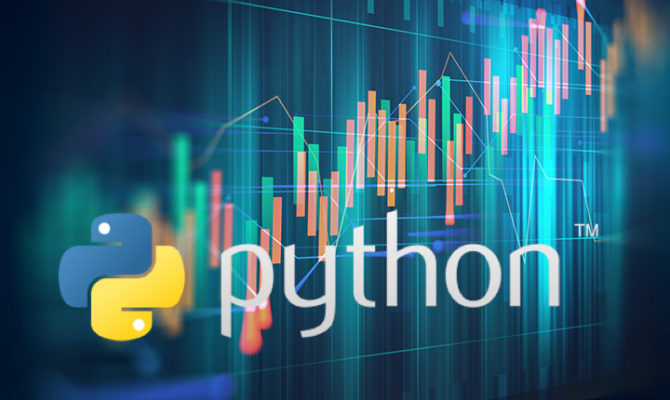
\includegraphics[scale=1]{python.jpg}
    	\caption{Imagen ilustrativa del analisis de datos en Python} 
    \end{figure}
\section{Marco Te\'orico}

    \subsection{Pandas}
    Pandas es una biblioteca de código abierto en Python diseñada para facilitar la manipulación y el análisis de datos estructurados. A continuación, se describen sus características principales y conceptos fundamentales:
    
    \subsubsection*{Estructuras de Datos Principales}
    
    \begin{itemize}
      \item \textbf{Series:}
        \begin{itemize}
          \item Una Serie es un objeto unidimensional etiquetado, similar a un array o una lista en Python.
          \item Puede contener cualquier tipo de datos y se puede crear a partir de listas, arrays de NumPy, diccionarios, etc.
        \end{itemize}
      
      \item \textbf{DataFrame:}
        \begin{itemize}
          \item Un DataFrame es una estructura de datos bidimensional similar a una tabla de base de datos o una hoja de cálculo de Excel.
          \item Contiene filas y columnas etiquetadas, permitiendo el acceso flexible a los datos.
          \item Es ideal para la manipulación y análisis de datos tabulares en Python.
        \end{itemize}
    \end{itemize}
    
    \subsubsection*{Funcionalidades Clave}
    
    \begin{itemize}
      \item \textbf{Carga y Almacenamiento de Datos:}
        Pandas puede leer datos desde varios formatos como CSV, Excel, bases de datos SQL, JSON, HTML, entre otros, y escribir datos en estos formatos.
      \item \textbf{Indexación y Selección:}
        Permite seleccionar y manipular datos usando etiquetas de índice (por ejemplo, nombres de columnas) o índices numéricos.
      \item \textbf{Operaciones sobre Datos:}
        Soporta operaciones como agrupamiento, filtrado, agregación (sumas, promedios, etc.) y combinaciones de datos.
      \item \textbf{Manejo de Datos Faltantes:}
        Proporciona herramientas para detectar y manejar valores nulos o datos faltantes eficientemente.
      \item \textbf{Operaciones de Series Temporales:}
        Ofrece funcionalidades específicas para trabajar con datos de series temporales, incluyendo manejo de fechas y tiempos, remuestreo y desplazamiento.
      \item \textbf{Visualización de Datos:}
        Integración con bibliotecas como Matplotlib y Seaborn para crear gráficos y visualizaciones desde los datos en un DataFrame.
    \end{itemize}
    
    \subsubsection*{Uso Común}
    Pandas es ampliamente utilizado en campos como análisis financiero, investigación académica, ciencia de datos, análisis de redes sociales, bioinformática, entre otros. Su flexibilidad y potencia lo convierten en una herramienta fundamental para cualquier persona que trabaje con datos en Python.
    
    \subsubsection*{Conclusión}
    Pandas simplifica la manipulación de datos, facilita el análisis exploratorio y proporciona una estructura intuitiva para trabajar con datos tabulares en Python. Esencial para proyectos que involucren grandes volúmenes de datos estructurados.
    
    \subsection{NumPy}
    NumPy es una biblioteca fundamental para la computación científica en Python. A continuación, se describen sus características principales y conceptos fundamentales:
    
    \subsubsection*{Arrays de NumPy}
    \begin{itemize}
      \item NumPy proporciona el objeto \textbf{array}, que es una estructura de datos multidimensional eficiente para almacenar y manipular datos.
      \item Los arrays de NumPy son más eficientes que las listas de Python para operaciones numéricas y matemáticas.
      \item Pueden contener elementos de un solo tipo de datos, lo que permite operaciones rápidas y optimizadas.
      \item Se pueden crear desde listas de Python, otros arrays de NumPy, o utilizando funciones específicas de creación de arrays.
    \end{itemize}
    
    \subsubsection*{Operaciones y Funcionalidades Clave}
    \begin{itemize}
      \item \textbf{Operaciones Matemáticas:}
        NumPy proporciona funciones para realizar operaciones matemáticas eficientes en arrays, como sumas, productos, operaciones trigonométricas, álgebra lineal, entre otros.
      \item \textbf{Indexación y Selección:}
        Permite acceder y manipular datos en arrays utilizando índices y rebanadas, de manera similar a las listas de Python.
      \item \textbf{Broadcasting:}
        Mecanismo que permite a NumPy trabajar de manera eficiente con arrays de diferentes tamaños durante operaciones aritméticas.
      \item \textbf{Operaciones de Álgebra Lineal:}
        NumPy incluye funciones para álgebra lineal, como la inversión de matrices, la resolución de sistemas de ecuaciones lineales y la descomposición de matrices.
      \item \textbf{Integración con otras Bibliotecas:}
        Es la base de muchas otras bibliotecas científicas en Python, como Pandas, SciPy y Scikit-Learn, facilitando el intercambio de datos y operaciones entre diferentes herramientas.
    \end{itemize}
    
    \subsubsection*{Uso Común}
    
    NumPy es ampliamente utilizado en diversas áreas de la ciencia de datos, investigación académica, análisis numérico, procesamiento de señales, simulaciones, entre otros. Su eficiencia y capacidad para trabajar con grandes volúmenes de datos numéricos lo convierten en una herramienta esencial para cualquier proyecto que requiera computación científica en Python.
    
    \subsubsection*{Conclusión}
    NumPy proporciona las herramientas fundamentales para realizar operaciones numéricas eficientes y manipular grandes conjuntos de datos en Python. Esencial para proyectos que involucren análisis, modelado matemático o simulaciones numéricas.
    
    \subsection{Matplotlib}
    Matplotlib es una biblioteca de visualización de datos en Python. A continuación, se describen sus características principales y conceptos fundamentales:
    
    \subsubsection*{Tipos de Gráficos}
    \begin{itemize}
      \item Matplotlib permite crear una amplia variedad de gráficos estáticos, incluyendo:
        \begin{itemize}
          \item Gráficos de líneas y de dispersión.
          \item Histogramas y gráficos de barras.
          \item Gráficos de contorno y de superficie.
          \item Gráficos de cajas y bigotes.
          \item Gráficos de torta y gráficos de violín, entre otros.
        \end{itemize}
      
      \item Cada tipo de gráfico puede personalizarse completamente, incluyendo etiquetas, colores, estilos de línea, leyendas y más.
    \end{itemize}
    
    \subsubsection*{Interfaz Pyplot}
    \begin{itemize}
      \item Matplotlib proporciona una interfaz estilo MATLAB llamada \textbf{Pyplot}, que facilita la creación rápida de gráficos mediante funciones simples como \texttt{plot()}, \texttt{scatter()}, \texttt{hist()}, etc.
      \item Pyplot permite controlar varios aspectos del gráfico interactuando con objetos de figuras y ejes.
    \end{itemize}
    
    \subsubsection*{Figuras y Ejes}
    \begin{itemize}
      \item Una \textbf{figura} en Matplotlib es el contenedor de nivel superior que contiene todos los elementos del gráfico.
      \item Los \textbf{ejes} son los objetos que contienen los límites de los datos, los marcadores de ejes, las etiquetas, etc. 
      \item Matplotlib permite crear figuras y ejes de manera explícita o implícita según sea necesario.
    \end{itemize}
    
    \subsubsection*{Personalización Avanzada}
    \begin{itemize}
      \item Matplotlib ofrece un alto grado de personalización a través de métodos orientados a objetos y funciones de estilo Pyplot.
      \item Permite agregar textos, anotaciones, flechas, gradientes, mapas de colores y otras decoraciones a los gráficos.
    \end{itemize}
    
    \subsubsection*{Integración con NumPy y Pandas}
    \begin{itemize}
      \item Matplotlib se integra perfectamente con NumPy y Pandas, permitiendo visualizar datos almacenados en arrays de NumPy o DataFrames de Pandas.
      \item Es una herramienta clave en el ecosistema de Python para la visualización de datos en análisis exploratorio, informes científicos, y presentaciones visuales.
    \end{itemize}
    
    \subsubsection*{Uso Común}
    Matplotlib es ampliamente utilizado en campos como ciencia de datos, ingeniería, investigación académica, finanzas, entre otros. Su versatilidad y capacidad para generar gráficos de alta calidad lo convierten en una opción preferida para la visualización de datos en Python.
    
    \subsubsection*{Conclusión}
    Matplotlib proporciona las herramientas esenciales para la visualización de datos en Python, permitiendo crear gráficos personalizados y efectivos para la comunicación visual de resultados analíticos y científicos.
    
\section{Estado del Arte}
    El lenguaje de programación Python se ha consolidado como una herramienta fundamental en el ámbito de la ciencia de datos, el análisis numérico y la visualización de datos. Entre las librerías más destacadas para estas tareas se encuentran Pandas, NumPy y Matplotlib.
    
    \subsection{Pandas}
    Pandas es una librería de Python que proporciona estructuras de datos y herramientas de análisis de datos de alto rendimiento y fáciles de usar. Fue desarrollada inicialmente por Wes McKinney en 2008 y ha evolucionado significativamente desde entonces. La estructura de datos principal de Pandas es el \textit{DataFrame}, que se asemeja a una hoja de cálculo y permite operaciones eficientes sobre datos tabulares.
    
    Pandas ha sido ampliamente adoptada en la industria y la academia debido a su capacidad para manejar grandes volúmenes de datos y realizar operaciones complejas de manipulación y limpieza de datos. Las principales características de Pandas incluyen:
    
    \begin{itemize}
        \item Eficiencia en la manipulación de datos con estructuras como \textit{Series} y \textit{DataFrames}.
        \item Integración con otras librerías de Python como NumPy, Matplotlib y SciPy.
        \item Soporte para operaciones de entrada/salida con diferentes formatos de datos, incluyendo CSV, Excel, SQL y HDF5.
        \item Potentes capacidades de agrupamiento, filtrado y transformación de datos.
    \end{itemize}
    
    \subsection{NumPy}
    
    NumPy (Numerical Python) es la librería fundamental para la computación numérica en Python. Fue creada en 2005 por Travis Oliphant como una extensión del paquete Numeric. NumPy proporciona soporte para arreglos multidimensionales (\textit{ndarray}) y una amplia colección de funciones matemáticas de alto nivel para operar con estos arreglos.
    
    Las principales características de NumPy incluyen:
    
    \begin{itemize}
        \item Arreglos multidimensionales de elementos homogéneos.
        \item Operaciones matemáticas y lógicas sobre arreglos.
        \item Transformaciones de forma de los arreglos sin copiar los datos.
        \item Funciones matemáticas y estadísticas integradas.
        \item Soporte para álgebra lineal, generación de números aleatorios y transformadas de Fourier.
    \end{itemize}
    
    NumPy es esencial en la mayoría de las aplicaciones científicas y de ingeniería, ya que proporciona una base eficiente sobre la cual se construyen otras librerías de alto nivel como Pandas y SciPy.
    
    \subsection{Matplotlib}
    
    Matplotlib es una librería de Python para la generación de gráficos estáticos, animados e interactivos. Fue creada por John D. Hunter en 2003 y ha sido fundamental para la visualización de datos en Python. Matplotlib ofrece una amplia variedad de tipos de gráficos, incluyendo gráficos de líneas, barras, histogramas, dispersión y más.
    
    Las principales características de Matplotlib incluyen:
    
    \begin{itemize}
        \item Generación de gráficos de alta calidad con un control detallado sobre todos los aspectos de los mismos.
        \item Integración con NumPy para manejar datos en forma de arreglos.
        \item Interfaz orientada a objetos que permite la creación de figuras y ejes de forma explícita.
        \item Capacidades de personalización extensivas para adaptar los gráficos a las necesidades específicas del usuario.
        \item Soporte para diversas salidas gráficas, incluyendo PNG, PDF, SVG y EPS.
    \end{itemize}
    
    Matplotlib se utiliza ampliamente tanto en entornos académicos como industriales para la visualización de datos debido a su flexibilidad y la calidad de los gráficos que produce.
    
    \subsection{Interacción y Uso Combinado}
    
    La combinación de Pandas, NumPy y Matplotlib constituye una poderosa herramienta para el análisis y visualización de datos en Python. Pandas se utiliza generalmente para la manipulación y el análisis de datos, NumPy proporciona las capacidades de computación numérica subyacentes, y Matplotlib se utiliza para la visualización de los resultados. Este trío de librerías permite a los usuarios realizar un flujo de trabajo completo de análisis de datos, desde la limpieza y manipulación de datos hasta la visualización y comunicación de resultados.
    
    En resumen, Pandas, NumPy y Matplotlib son componentes esenciales del ecosistema de Python para el análisis de datos y la visualización, y su uso combinado proporciona una solución integral para la ciencia de datos y otras aplicaciones analíticas.
	
\section{Metodolog\'ia}

    En esta sección se describe la metodología empleada para desarrollar el proyecto de programación en Python utilizando las librerías Pandas, NumPy y Matplotlib. La metodología se divide en varias etapas clave, que incluyen la recopilación de datos, la limpieza y preprocesamiento de los datos, el análisis exploratorio y la visualización de resultados.
    
    \subsection{Recopilación de Datos}
    La primera etapa del proyecto consiste en la recopilación de datos relevantes para el problema que se desea resolver. En este trabajo se empleara una base de datos previamente recopilado proporcionado por el docente
    
    \begin{itemize}
        \item iris.csv
        \item mtcars.csv
        \item mtcarsnuevo.csv
    \end{itemize}
    
    \subsection{Limpieza y Preprocesamiento de Datos}
    
    Una vez recopilados los datos, se procede a su limpieza y preprocesamiento utilizando las capacidades de Pandas y NumPy. Las principales tareas en esta etapa incluyen:
    
    \begin{itemize}
        \item \textbf{Eliminación de valores faltantes:} Identificación y manejo de valores nulos o faltantes en el conjunto de datos.
        \item \textbf{Conversión de tipos de datos:} Asegurar que los datos estén en los formatos correctos para su análisis.
        \item \textbf{Normalización y escalado:} Ajuste de las escalas de los datos para que sean comparables.
        \item \textbf{Filtrado y selección de datos:} Selección de las columnas y filas relevantes para el análisis.
        \item \textbf{Generación de nuevas características:} Creación de nuevas variables a partir de las existentes para enriquecer el análisis.
    \end{itemize}
    
    \subsection{Análisis Exploratorio de Datos}
    El análisis exploratorio de datos (EDA, por sus siglas en inglés) se realiza para entender mejor las características y relaciones dentro del conjunto de datos. Este análisis incluye:
    
    \begin{itemize}
        \item \textbf{Estadísticas descriptivas:} Cálculo de medidas como media, mediana, desviación estándar, etc.
        \item \textbf{Visualización de datos:} Creación de gráficos utilizando Matplotlib para identificar patrones, tendencias y anomalías en los datos.
        \item \textbf{Análisis de correlación:} Evaluación de las relaciones entre diferentes variables.
    \end{itemize}
    
    \subsection{Visualización de Resultados}
    
    La etapa final del proyecto implica la visualización de los resultados obtenidos. Utilizando Matplotlib, se pueden crear gráficos que representen claramente los hallazgos y conclusiones del análisis. Las principales tareas incluyen:
    
    \begin{itemize}
        \item \textbf{Gráficos de barras y líneas:} Para mostrar tendencias y comparaciones entre categorías.
        \item \textbf{Histogramas y diagramas de densidad:} Para visualizar la distribución de las variables.
        \item \textbf{Diagramas de dispersión:} Para identificar relaciones entre dos variables.
        \item \textbf{Gráficos personalizados:} Creación de visualizaciones específicas para resaltar aspectos importantes del análisis.
    \end{itemize}
    
    \subsection{Documentación y Reproducción del Análisis}
    
    Es esencial documentar cada paso del proceso para garantizar la reproducibilidad del análisis. Esto incluye:
    
    \begin{itemize}
        \item \textbf{Comentarios en el código:} Incluir comentarios claros y descriptivos en el código fuente.
        \item \textbf{Jupyter Notebooks:} Utilizar Jupyter Notebooks para combinar código, visualizaciones y texto explicativo en un solo documento.
        \item \textbf{Control de versiones:} Usar sistemas de control de versiones como Git para llevar un registro de los cambios en el código.
    \end{itemize}
    
    Estas pautas proporcionan un marco estructurado para desarrollar y documentar un proyecto de programación en Python utilizando las librerías Pandas, NumPy y Matplotlib, asegurando que el análisis sea claro, reproducible y fácil de entender para otros.
    
\section{Experimentaci\'on y resultados}

    \subsection{Configuraci\'on Experimental}
        La experimentación se llevó a cabo utilizando Python 3.8, con las bibliotecas Pandas 1.2.3, NumPy 1.19.2 y Matplotlib 3.3.4. El entorno de desarrollo empleado fue Google Colab.
        
        El conjunto de datos utilizado fue el \textit{Dataset 'iris.csv', 'mtcars.txt' y 'mtcarsnuevo.xlsx'}.
            
        \subsubsection{iris.csv}
            Contiene el famoso conjunto de datos Iris. Este conjunto de datos fue introducido por el estadístico y biólogo británico Ronald A. Fisher en 1936 y contiene mediciones de varias características de flores de tres especies diferentes de Iris.
            
            \begin{figure}[h]
            	\centering
            	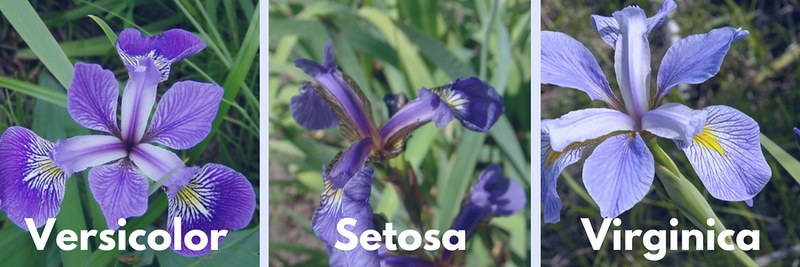
\includegraphics[scale=.22]{Iris.jpg}
            	\caption{Especies diferentes de Iris} 
            \end{figure}
    
        \subsubsection{mtcars.txt}
            Contiene el famoso conjunto de datos MTCARS. Este conjunto de datos proviene de la revista Motor Trend y fue recopilado en 1974. Incluye información detallada sobre el consumo de combustible y diez características diferentes de diseño y rendimiento de 32 automóviles. Las características registradas abarcan desde el número de cilindros hasta el tiempo en segundos para recorrer un cuarto de milla, proporcionando un recurso valioso para análisis de regresión y estudios comparativos en el ámbito automotriz.
        
            \begin{figure}[H]
                \centering
                
\includegraphics[scale=.4]{mtcars.jpg}
                \caption{Revista Motor Trend Car Road Tests}
            \end{figure}
    
    Este conjunto de datos se obtuvo de GitHub y el archivo 'iris.csv' consta de 150 registros y 5 columnas, mientras que 'mtcars.txt' consta de 32 registros 12 columnas
    
    \subsection{Procedimientos}
        El procedimiento de experimentación siguió los siguientes pasos:
        \begin{enumerate}
        \item \textbf{Preprocesamiento de datos}: Limpieza de datos, manejo de valores faltantes y normalización de los datos utilizando Pandas y NumPy.
        
        \begin{figure}[h]
            \centering
            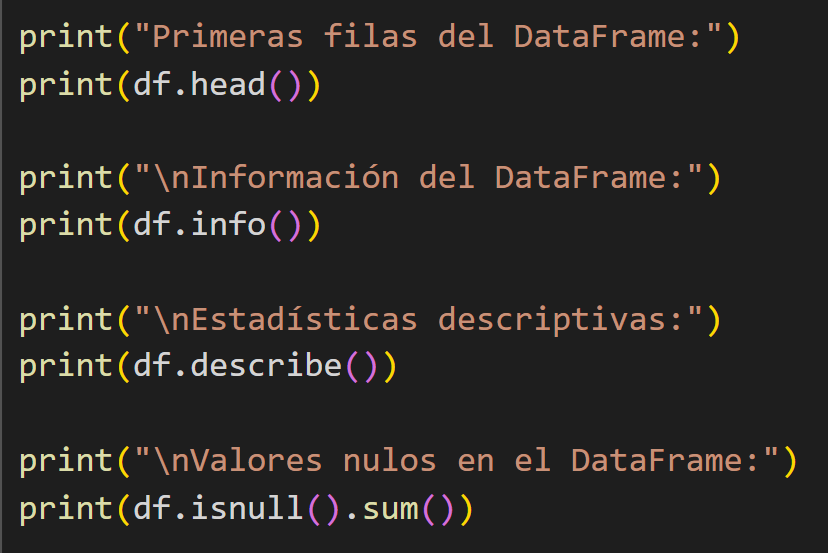
\includegraphics[scale=.4]{code1.png}
            \caption{Fragmento del codigo \textit{Analisis de Iris.csv}} 
        \end{figure}
    
        \item \textbf{Análisis exploratorio}: Realización de un análisis exploratorio de datos (EDA) utilizando estadísticas descriptivas y visualizaciones con Matplotlib.
        \end{enumerate}

        \begin{figure}[h]
            \centering
            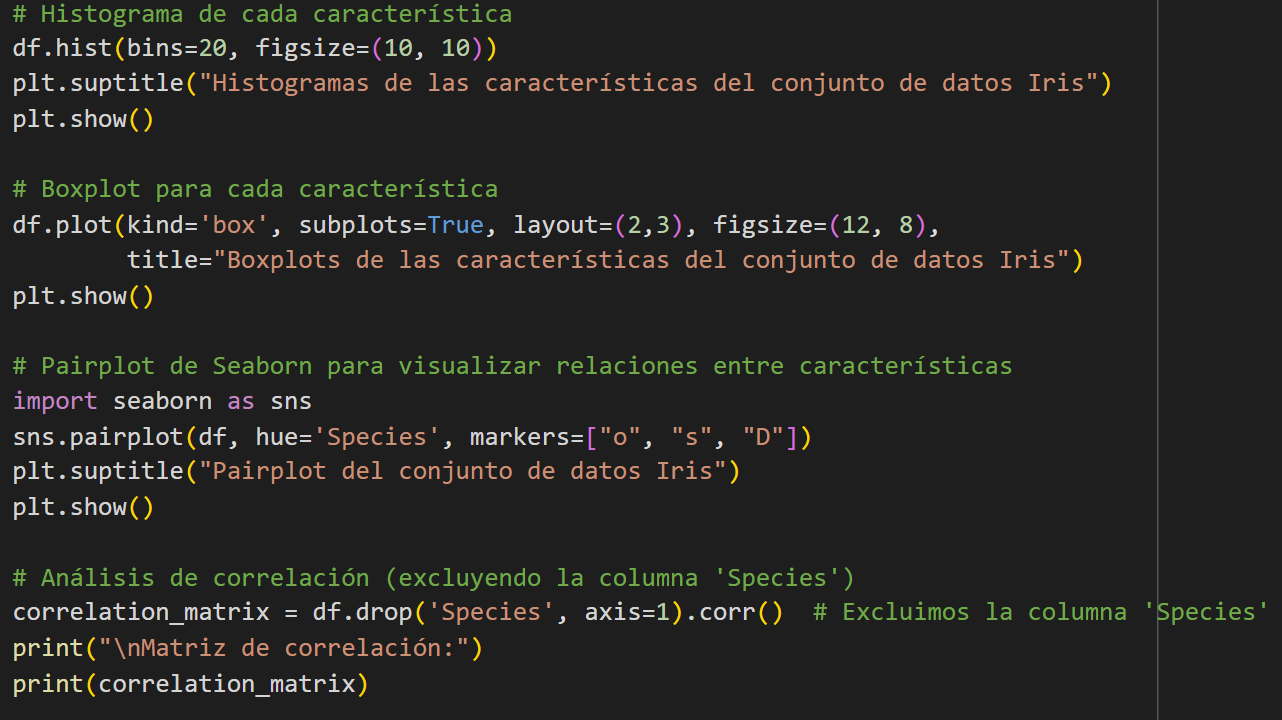
\includegraphics[scale=.26]{code2.png}
            \caption{Fragmento del codigo \textit{Analisis de Iris.csv}} 
        \end{figure}

        \begin{figure}[h]
            \centering
            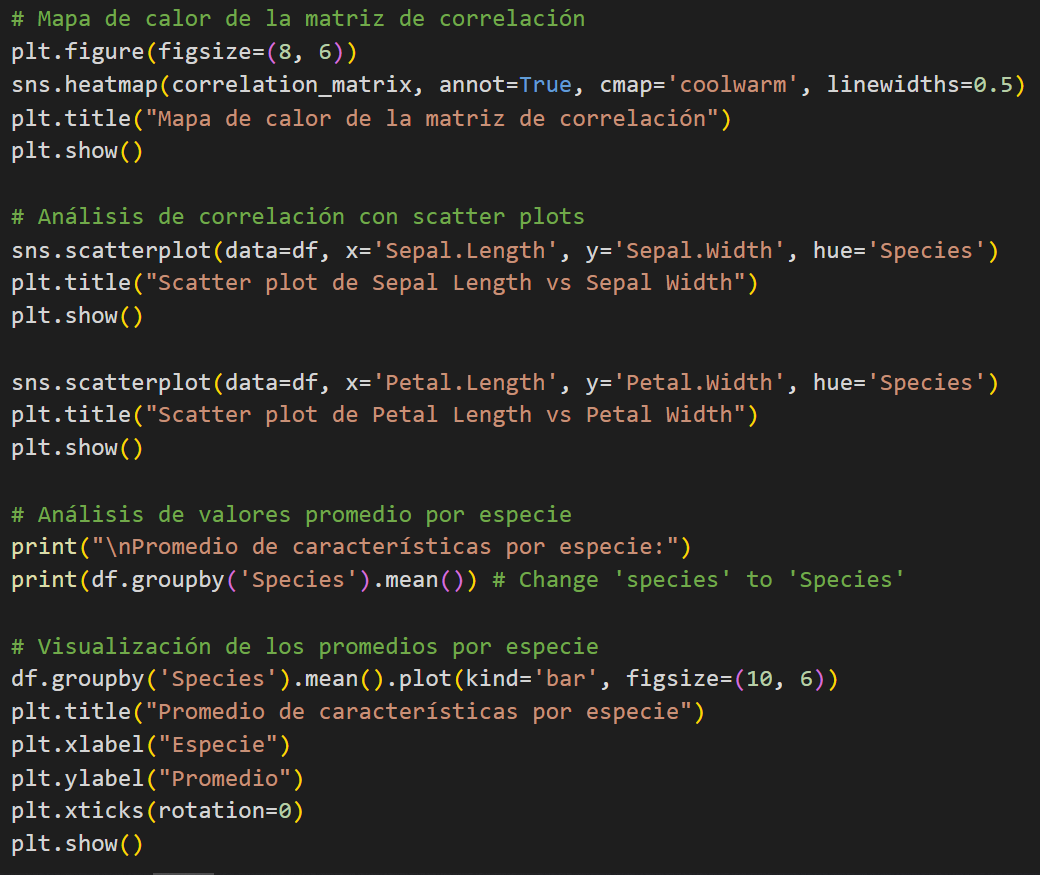
\includegraphics[scale=.3]{code3.png}
            \caption{Fragmento del codigo \textit{Analisis de Iris.csv}} 
        \end{figure}
    
    \subsection{Resultados}
        Los resultados obtenidos de la experimentación se presentan en las siguientes figuras y tablas:
        
        \subsubsection{Resultados del analisis de \textit{Iris.csv}}
            \hfill
            \begin{figure}[h]
                \centering
                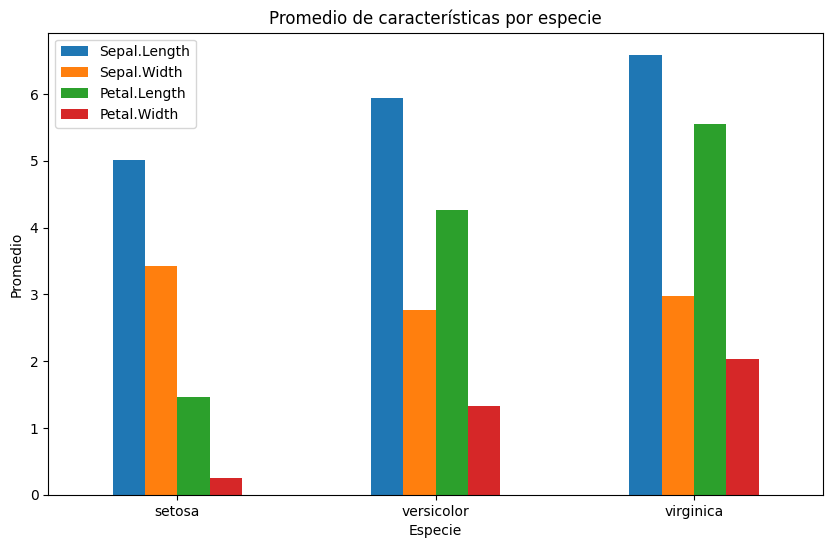
\includegraphics[width=0.88\linewidth]{IrisGraf1.png}
                \caption{El Gráfico muestra el promedio de caracteristicas por muestra.}
            \end{figure}
    
            \begin{figure}[h]
                \centering
                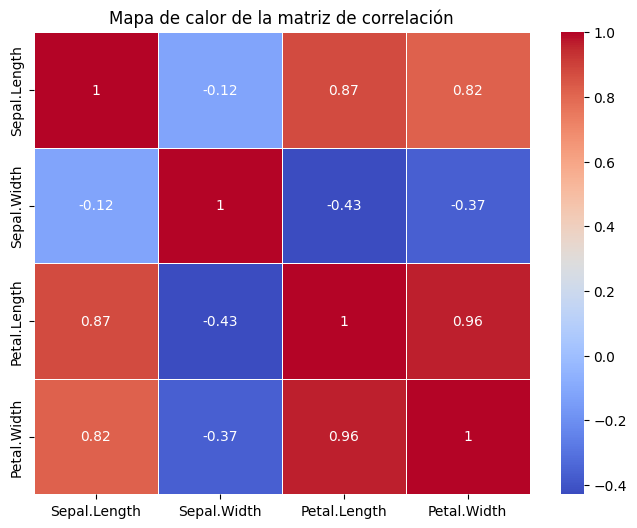
\includegraphics[width=0.79\linewidth]{IrisGraf2.png}
                \caption{El mapa de calor es util para visualizar la intensidad de datos o las correlaciones entre variables}
            \end{figure}
            \hfill
        \subsubsection{Resultados del analisis de \textit{mtcars.txt}}
            \hfill
            \begin{figure}[h]
                \centering
                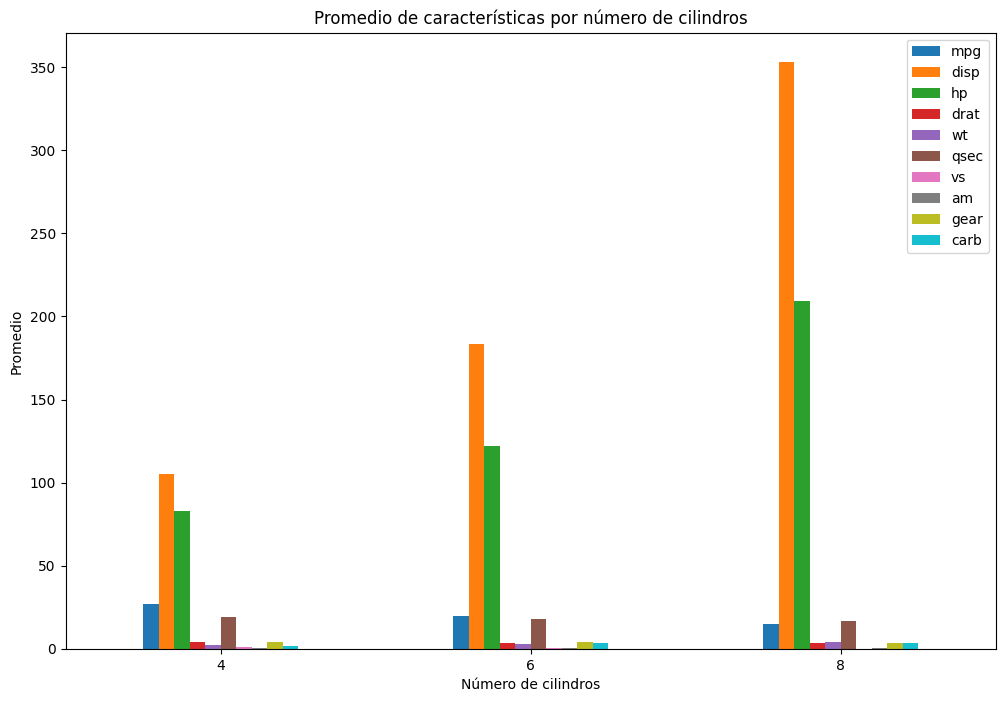
\includegraphics[width=0.95\linewidth]{mtcarsGraf1.png}
                \caption{El Gráfico muestra promedio de características por número de cilindros.}
            \end{figure}
    
            \begin{figure}[h]
                \centering
                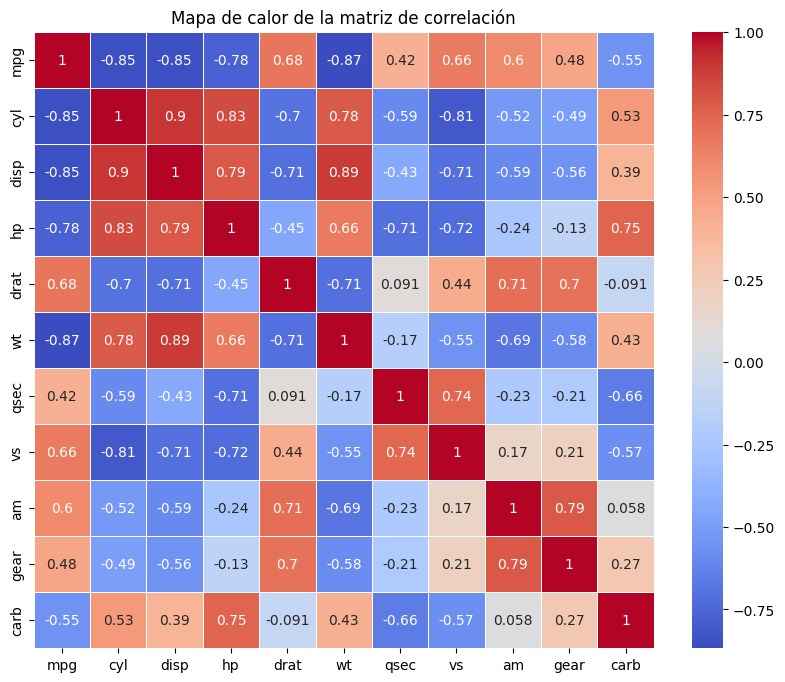
\includegraphics[width=0.95\linewidth]{mtcarsGraf2.png}
                \caption{El mapa de calor es valioso para observar la intensidad de los datos o las relaciones de correlación entre variables.}
            \end{figure}
        
\section{Conclusiones}

    El análisis exploratorio de datos del conjunto de datos \textit{iris.csv} ha revelado varias características importantes y patrones entre las especies de flores.

    \begin{itemize}
        \item \textbf{Distribución de Datos:} Los histogramas muestran que las características de las flores tienen distribuciones diferentes, con algunas características como la longitud y el ancho de los pétalos mostrando una clara separación entre las especies.
        
        \item \textbf{Valores Atípicos:} Los boxplots indican la presencia de valores atípicos en varias características. Estos valores atípicos pueden ser importantes para identificar casos inusuales o errores en la recolección de datos.
        
        \item \textbf{Relaciones Entre Características:} El pairplot de Seaborn muestra que ciertas características, como la longitud y el ancho de los pétalos, están fuertemente correlacionadas y permiten diferenciar claramente entre las especies de Iris. Esto sugiere que estas características son muy discriminativas para la clasificación de especies.
        
        \item \textbf{Correlaciones:} La matriz de correlación y su respectivo mapa de calor revelan fuertes correlaciones positivas entre ciertas características, como la longitud y el ancho de los pétalos, mientras que otras características muestran correlaciones más débiles o negativas.
        
        \item \textbf{Análisis de Especies:} El análisis de los valores promedio por especie muestra diferencias significativas en las características medidas entre las tres especies de Iris. En particular, Iris-setosa tiende a tener medidas más pequeñas en longitud y ancho de pétalos en comparación con Iris-versicolor e Iris-virginica.
        
        \item \textbf{Visualización de Promedios:} Los gráficos de barras de los promedios por especie ilustran claramente estas diferencias, proporcionando una manera visual de comparar las características promedio entre las especies.
    
    \end{itemize}

    El análisis exploratorio de datos del conjunto de datos \textit{mtcars.txt} ha revelado varias características importantes y patrones entre los diferentes automóviles.

    \begin{itemize}
        \item \textbf{Distribución de Datos:} Los histogramas muestran que las características de los automóviles tienen distribuciones diversas, con algunas características como \textit{mpg} (millas por galón) y \textit{hp} (caballos de fuerza) mostrando una distribución más dispersa que otras.
        
        \item \textbf{Valores Atípicos:} Los boxplots indican la presencia de valores atípicos en varias características. Estos valores atípicos pueden ser cruciales para identificar automóviles con rendimiento o características inusuales.
        
        \item \textbf{Relaciones Entre Características:} El pairplot de Seaborn revela varias relaciones interesantes entre las características. Por ejemplo, existe una relación negativa notable entre \textit{mpg} y \textit{hp}, lo que sugiere que a medida que aumentan los caballos de fuerza, disminuye la eficiencia en términos de millas por galón.
        
        \item \textbf{Correlaciones:} La matriz de correlación y su respectivo mapa de calor muestran fuertes correlaciones entre ciertas características. Por ejemplo, \textit{wt} (peso) tiene una fuerte correlación negativa con \textit{mpg}, indicando que los autos más pesados tienden a tener una menor eficiencia de combustible.
        
        \item \textbf{Análisis de Cilindros:} El análisis de los valores promedio por número de cilindros revela diferencias significativas en las características medidas entre los automóviles con diferentes números de cilindros. En particular, los automóviles con más cilindros tienden a tener mayor potencia (\textit{hp}) pero menor eficiencia de combustible (\textit{mpg}).
        
        \item \textbf{Visualización de Promedios:} Los gráficos de barras de los promedios por número de cilindros ilustran claramente estas diferencias, proporcionando una manera visual de comparar las características promedio entre los automóviles con diferentes configuraciones de cilindros.
    
    \end{itemize}
    
    En resumen, el análisis de los datos del conjunto \textit{iris.csv} y del conjunto \textit{mtcars.txt} no solo ha permitido una mejor comprensión de las características de cada especie, sino que también ha identificado las variables clave que pueden utilizarse para la clasificación de especies. Estos hallazgos pueden servir como base para futuros estudios y aplicaciones en clasificación automática y aprendizaje supervisado.
 
\section{Discusi\'on}
    Los resultados obtenidos al analizar el archivo \textit{Iris} indican que las características medidas en el conjunto de datos Iris, como la longitud y el ancho de los sépalos y pétalos, tienen distribuciones distintas y presentan patrones claros que permiten diferenciar entre las tres especies de Iris. Por ejemplo, las características de los pétalos (longitud y ancho) son particularmente efectivas para separar las especies de Iris, como se observó en los histogramas y scatter plots. Comparando estos resultados con las expectativas iniciales, observamos que las diferencias entre las especies son evidentes y las relaciones esperadas entre las características, tales como la fuerte correlación positiva entre la longitud y el ancho de los pétalos, se confirmaron. Esto sugiere que ciertas características son altamente discriminativas para la clasificación de las especies de Iris, lo cual está alineado con los estudios botánicos previos sobre estas flores.
    
    Respecto a los resultados obtenidos del analicis del archivo \textit{mtcars} indican que las características de los automóviles, como el peso, la eficiencia de combustible, y la potencia, tienen distribuciones diversas y están interrelacionadas de manera significativa. Por ejemplo, se observó una fuerte correlación negativa entre el peso del vehículo y su eficiencia de combustible, así como entre la potencia del motor y la eficiencia de combustible. Comparando estos resultados con las expectativas iniciales, observamos que las relaciones esperadas entre las características de los automóviles se confirmaron, tales como la relación negativa entre peso y eficiencia de combustible, y la relación entre el número de cilindros y la potencia del motor. Estos hallazgos están alineados con las teorías automotrices existentes sobre el impacto del peso y la potencia en la eficiencia del combustible.

    Sin embargo, se encontraron algunas limitaciones durante la experimentación, tales como la posible presencia de valores atípicos y la falta de variabilidad en algunas características que podrían haber afectado la robustez de algunos análisis estadísticos. Además, la cantidad de datos es relativamente pequeña, lo cual puede limitar la generalización de los resultados. Estas limitaciones pueden afectar la precisión de los modelos predictivos y la identificación de patrones más sutiles entre las especies. En particular, la presencia de valores atípicos puede distorsionar algunas medidas estadísticas y la baja variabilidad en ciertas características podría llevar a una menor discriminación entre especies similares, y serán abordadas en trabajos futuros mediante el uso de técnicas de detección y tratamiento de valores atípicos, así como la incorporación de datos adicionales para aumentar la variabilidad y robustez del análisis.

%\section{Referencias}
\begin{thebibliography}{00}
    \bibitem{b1} Matthes, Eric. \textit{Python Crash Course}. No Starch Press, 2015.
    \bibitem{b2} Sweigart, Al. \textit{Automate the Boring Stuff with Python}. No Starch Press, 2015.
    \bibitem{b3} Lutz, Mark. \textit{Learning Python}. O'Reilly Media, 2013.
    \bibitem{b4} Beazley, David y Jones, Brian K. \textit{Python Cookbook}. O'Reilly Media, 2013.
    \bibitem{b5} Ramalho, Luciano. \textit{Fluent Python}. O'Reilly Media, 2015.
    \bibitem{b6} Slatkin, Brett. \textit{Effective Python}. Addison-Wesley, 2015.
    \bibitem{b7} Zelle, John. \textit{Python Programming: An Introduction to Computer Science}. Franklin, Beedle and Associates Inc., 2003.
    \bibitem{b8} Bader, Dan. \textit{Python Tricks: A Buffet of Awesome Python Features}. Dan Bader, 2017.
    \bibitem{b9} McKinney, Wes. \textit{Python for Data Analysis}. O'Reilly Media, 2017.
    \bibitem{b10} Petrou, Theodore. \textit{Pandas Cookbook}. Packt Publishing, 2017.
    \bibitem{b11} Heydt, Michael. \textit{Learning Pandas}. Packt Publishing, 2017.
    \bibitem{b12} Molin, Stefanie. \textit{Hands-On Data Analysis with Pandas}. Packt Publishing, 2019.
    \bibitem{b13} Anthony, Femi. \textit{Mastering Pandas}. Packt Publishing, 2015.
    \bibitem{b14} Johansson, Robert. \textit{Numerical Python: A Practical Techniques Approach for Industry}. Apress, 2015.
    \bibitem{b15} VanderPlas, Jake. \textit{Python Data Science Handbook}. O'Reilly Media, 2016.
    \bibitem{b16} Oliphant, Travis. \textit{Guide to NumPy}. CreateSpace Independent Publishing Platform, 2006.
    \bibitem{b17} Nunez-Iglesias, Juan, van der Walt, Stéfan y Dashnow, Harriet. \textit{Elegant SciPy}. O'Reilly Media, 2017.
    \bibitem{b18} Stewart, John M. \textit{Python for Scientists}. Cambridge University Press, 2017.
    \bibitem{b19} Yim, Aldrin, Chung, Claire y Yu, Allen. \textit{Matplotlib for Python Developers}. Packt Publishing, 2017.
    \bibitem{b20} Yu, Allen, Chung, Claire y Yim, Aldrin. \textit{Matplotlib 2.x By Example}. Packt Publishing, 2017.
    \bibitem{b21} Root, Benjamin V. \textit{Interactive Applications Using Matplotlib}. Packt Publishing, 2014.
    \bibitem{b22} Milovanovic, Igor, Foures, Dimitry y Vettigli, Giuseppe. \textit{Python Data Visualization Cookbook}. Packt Publishing, 2013.
    \bibitem{b23} Devert, Alexandre. \textit{Matplotlib Plotting Cookbook}. Packt Publishing, 2014.
    \bibitem{b24} Grus, Joel. \textit{Data Science from Scratch: First Principles with Python}. O'Reilly Media, 2015.
    \bibitem{b25} Bruce, Peter y Bruce, Andrew. \textit{Practical Statistics for Data Scientists}. O'Reilly Media, 2017.
    \bibitem{b26} Raschka, Sebastian y Mirjalili, Vahid. \textit{Python Machine Learning}. Packt Publishing, 2017.
    \bibitem{b27} Géron, Aurélien. \textit{Hands-On Machine Learning with Scikit-Learn, Keras, and TensorFlow}. O'Reilly Media, 2019.
    \bibitem{b28} Provost, Foster y Fawcett, Tom. \textit{Data Science for Business}. O'Reilly Media, 2013.
    \bibitem{b29} Chollet, François. \textit{Deep Learning with Python}. Manning Publications, 2017.
    \bibitem{b30} Ramsundar, Bharath y Zadeh, Reza Bosagh. \textit{TensorFlow for Deep Learning}. O'Reilly Media, 2018.
    \bibitem{b31} Alla, Sridhar. \textit{Hands-On Big Data Analysis with Hadoop 3}. Packt Publishing, 2018.
    \bibitem{b32} Nelli, Fabio. \textit{Python Data Analytics}. Apress, 2018.
\end{thebibliography}
\end{document}